% !TEX encoding = UTF-8
% !TEX program = xelatex
\documentclass[12pt,a4paper]{article}
\usepackage[paperwidth=210mm, paperheight=297mm, left=0.75in, right=0.75in, bottom=1in, top=1in]{geometry}
\usepackage{polyglossia}
\setdefaultlanguage[babelshorthands]{italian}
\usepackage{fontspec}
\usepackage{graphicx}
\usepackage{blindtext}
\usepackage{wrapfig}

\frenchspacing
\makeindex

\begin{document}
\title{\vspace{-70pt}Herschell}
\author{Federico Bignoni}
\date{}
\maketitle
\pagestyle{empty}
\thispagestyle{empty}

\section*{Storia}
\label{storia}
\begin{wrapfigure}{r}{0.35\textwidth}
  \vspace{-10pt}
  \begin{center}
    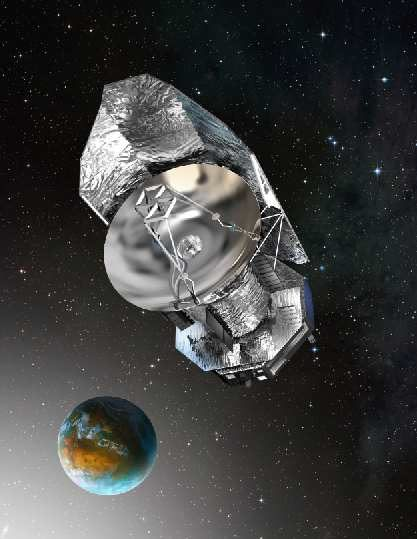
\includegraphics[width=0.30\textwidth]{satellite}
  \end{center}
  \vspace{-20pt}
\end{wrapfigure}
L'Herschel Space Observatory è una missione dell'Agenzia Spaziale Europea.
È stata lanciata il 14 maggio 2009 alle 13:12 GMT insieme al Planck Surveyor.
Il telescopio è posizionato a 1,5 milioni di chilometri di distanza dalla Terra su un'orbita di Lissajous nel secondo punto di Lagrange del sistema Sole-Terra, da dove ha raccolto informazioni sull'aspetto dell'universo nell'infrarosso. Il 29 aprile 2013 alle 14:49:23 (UTC) il telescopio ha terminato la sua riserva di elio[1], la cui evaporazione permetteva di mantenere gli strumenti ad una temperatura prossima allo zero assoluto, rendendolo cieco.

Il Telescopio spaziale Herschel è il primo osservatorio spaziale a coprire tutte le lunghezze d'onda dell'infrarosso e submillimetriche. Il telescopio ha un ampio specchio dispiegato nello spazio (largo tre metri e mezzo).

L'osservatorio si specializzerà nell'osservazione degli oggetti poco conosciuti in particolare delle galassie neonate a migliaia o milioni di anni luce.

\section{Osservazioni}
\label{osservazioni}

Obiettivi della missione : 

\begin{itemize}
\item Studiare la formazione delle galassie nell'universo primordiale e l'evoluzione seguente.

\item Studiare la formazione delle stelle e la loro interazione con le polveri interstellari

\item Osservare la composizione chimica e l'atmosfera e la superficie delle comete, dei pianeti e dei satelliti.

\item Esaminare la chimica molecolare dell'Universo.

\end{itemize}

\section{Curiosità}
\label{curiosit}

La radiazione infrarossa viene focalizzata da tre strumenti i cui sensori sono mantenuti a meno di 2 K:

\begin{itemize}
\item PACS (Photodetecting Array Camera and Spectrometer)
Una fotocamera e spettrometro a bassa risoluzione che copre la banda tra 55 e 210 micrometri.

\item SPIRE (Spectral and Photometric Imaging Receiver)
Una fotocamera e spettrometro a bassa risoluzione che copre la banda tra 194 e 672 micrometri. 

\item HIFI (Heterodyne Instrument for the Far Infrared)
Un sensore con risoluzione spettrale fino a 107 micrometri. 

\end{itemize}


\end{document}